% ============================================================
%  HALAMAN PERNYATAAN ORISINALITAS DAN PUBLIKASI
%  Pedoman: TNR 12pt, spasi 1.5, justify
% ============================================================
\thispagestyle{chapterpage}
\phantomsection
\addcontentsline{toc}{chapter}{PERNYATAAN ORISINALITAS DAN PUBLIKASI}
\pagestyle{chapterpage}

\begin{center}
  {\bfseries\fontsize{12}{14}\selectfont
  PERNYATAAN ORISINALITAS DAN PUBLIKASI}
\end{center}

\vspace{2\baselineskip}

Saya yang bertanda tangan di bawah ini,

\vspace{1\baselineskip}

\noindent
\begin{tabular}{p{3.5cm} c p{9cm}}
  Nama            & : & \NamaMahasiswa \\[0.5em]
  NPM             & : & \NPM \\[0.5em]
  Judul PI        & : & \JudulPISatu \\[0.5em]
  Tanggal Sidang  & : & \TanggalSidang \\[0.5em]
  Tanggal Lulus   & : & \TanggalLulus \\
\end{tabular}

\vspace{1\baselineskip}

\noindent
menyatakan bahwa tulisan ini adalah merupakan hasil karya saya sendiri dan dapat
dipublikasikan sepenuhnya oleh Universitas Gunadarma. Segala kutipan dalam bentuk
apa pun telah mengikuti kaidah, etika yang berlaku. Mengenai isi dan tulisan adalah
merupakan tanggung jawab Penulis, bukan Universitas Gunadarma. Demikian pernyataan
ini dibuat dengan sebenarnya dan dengan penuh kesadaran.

\vspace{1\baselineskip}

\noindent
\begin{minipage}[t]{0.35\textwidth}
  \raisebox{-\height}{% <-- turunkan fbox agar baseline-nya di atas
    \fbox{\begin{minipage}[c][4.2cm][c]{3.2cm}
            \centering
            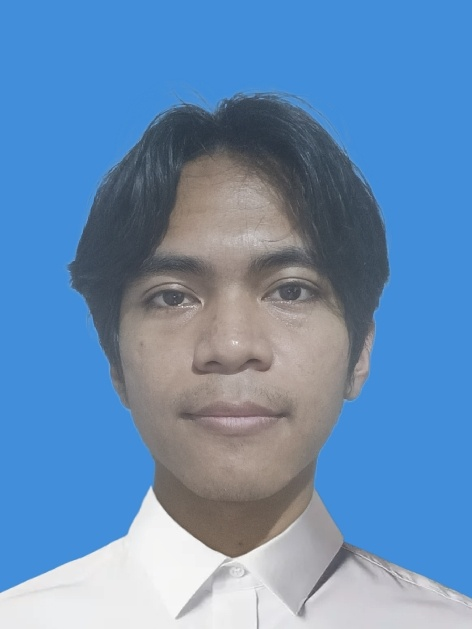
\includegraphics[width=3cm,height=4cm,keepaspectratio]{gambar/passphoto}
    \end{minipage}}%
  }
\end{minipage}
\hfill
\begin{minipage}[t]{0.55\textwidth}
  \vspace{0.02cm}
  Jakarta, \TanggalACC

  \vspace{0.5cm}


  
\includegraphics[width=3cm]{gambar/signature}\\[-0.3em]
  (\NamaMahasiswa)
\end{minipage}

\newpage
\pagestyle{chapterpage}
